%******************************************************************************%
%                                                                              %
%                  sample.en.tex for LaTeX                                     %
%                  Created on : Tue Mar 10 13:27:28 2015                       %
%                  Made by : David "Thor" GIRON <thor@42.fr>                   %
%                                                                              %
%******************************************************************************%

\documentclass{42-en}


%******************************************************************************%
%                                                                              %
%                                    Header                                    %
%                                                                              %
%******************************************************************************%
\begin{document}
				
				
		\title{Object Oriented Programming, Part 3 - Stacks and Queues}
        \subtitle{(In the beginning, there was Stack Overflow)}
	\member{Pragathi N}{pragathi.code@gmail.com}
	\member{Ted Tran}{42hourai@gmail.com}

\summary {
	This PDF is an introduction to \texttt{stacks} and \texttt{queues} in Python.
}

\maketitle

\tableofcontents


%******************************************************************************%
%                                                                              %
%                                  Foreword                                    %
%                                                                              %
%******************************************************************************%
\chapter{Foreword}

	Leptodactylus fallax, commonly (and deceptively) known as the mountain 
	chicken or giant ditch frog, is a species of frogs that is native to the
	Caribbean islands of Dominica and Montserrat. The population has declined 
	81\% in the last ten years and this species is now critically endangered. 
	In 2004 it was estimated that the population possibly was as low as 8,000 individuals.
	One of the main threats is human consumption. \\
	
	Being deliciously chicken-tasting is dangerous. \\

%******************************************************************************%
%                                                                              %
%                                  Goals                                       %
%                                                                              %
%******************************************************************************%
\chapter{Goals}

	\begin{itemize}
		\item Review stacks and queues.
		\item Write your own stack and queue classes.
		\item Practice using stacks and queues to accomplish a variety of tasks
	\end{itemize}


%******************************************************************************%
%                                                                              %
%                                 Introduction                                 %
%                                                                              %
%******************************************************************************%
\chapter{Introduction}

    Prepare to work with stacks and queues!\\
    These two are linear data structures that acts like a container of objects. 
    Difference between the two data structures is in the way the elements are accessed.

    \texttt{Stacks:} LIFO and \texttt{Queues:} FIFO

    If you don't know what LIFO means, google it! Or bother Pragathi, her number
    is 1-888-447-5594. If you want someone nicer, call 605-475-6966!\\

	           \begin{figure}[H]
		       \begin{center}
			       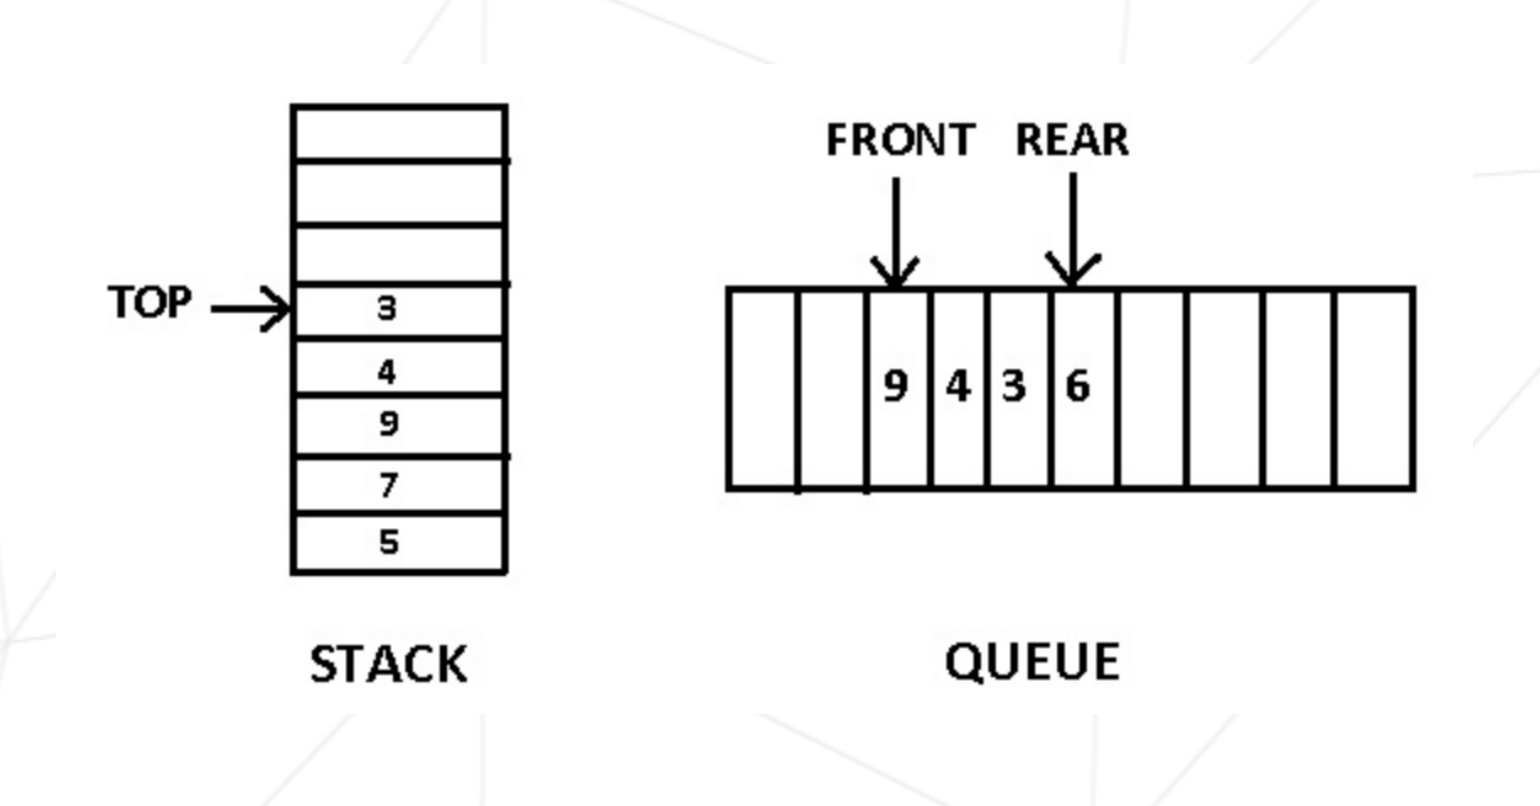
\includegraphics[width=15cm]{images/intro.png}
			\end{center}
		   \end{figure}


% Don't forget this line for piscine days to initate the exercise counter at 0
\startexercices

%******************************************************************************%
%                                                                              %
%                             Day of the Piscine                               %
%                                                                              %
%******************************************************************************%

\chapter{Exercise \exercicenumber: Stack Creation}

\extitle{Stack Creation}
\exnumber{\exercicenumber}
\exfiles{stack.py}

\makeheaderfiles

Make use of the Node class for the elements of the stack\\
            	\begin{figure}[H]
                	\begin{center}
                    		\includegraphics[width=10cm]{images/listNode.png}
                	\end{center}
            	\end{figure}

Implement a stack class with the following methods: \\
        	\begin{description}\itemsep3pt
			\item [def \_\_init\_\_(self):] Initialize the stack class with required variables 
			\item [def isEmpty(self):] Checks if the stack is empty or not (return None if empty) 
			\item [def push(self, data):] Adds an element to the stack
			\item [def pop(self):] removes the top element from the stack
			\item [def peek(self):] returns the value of the top element of the stack
			\item [def size(self):] returns the size of the stack
			\item [def \_\_str\_\_(self):] prints the elements of the stack\\
        	\end{description}

\nextexercice

\chapter{Exercise \exercicenumber: Basic Arithmetic}

\extitle{Basic Arithmetic}
\exnumber{\exercicenumber}
\exfiles{math.py}

\makeheaderfiles

Input a list and create a stack of the elements in the given list and implement the following operations on the stack. 
Start from the top of the stack when doing operations! Print the values in the same order as functions \\

		\begin{itemize}\itemsep1pt
			\item Calculate the total number of elements in the stack.
			\item Calculate the sum of all the elements in the stack.
			\item Multiply all the elements in the stack.
			\item Find the mean of the stack
			\item Lastly, find the maximum and minimum elements of the stack.
        	\end{itemize}
		
		\begin{42console}
			?> python math.py
			Enter the numbers: 1, 2, 3, 4, 5, 6, 7, 8, 9, 10
			Total count = 10
			Sum = 55
			Product = 3628800
			Mean = 5
			Min = 1
			Max = 10
		\end{42console}

\chapter{Exercise \exercicenumber: Queue Creation}

\extitle{Queue Creation}
\exnumber{\exercicenumber}
\exfiles{queue.py}

\makeheaderfiles

Make use of the Node class for the elements of the queue\\
            	\begin{figure}[H]
                	\begin{center}
                    		\includegraphics[width=10cm]{images/listNode.png}
                	\end{center}
            	\end{figure}

Implement a queue class with the following methods: \\
        	\begin{description}\itemsep1pt
			\item [def \_\_init\_\_(self):] Initialize the queue class with required variables (Front stores the
			front node and rear stores the last node)
			\item [def isEmpty(self):] Checks if the queue is empty or not (return None if empty) 
			\item [def enqueue(self, data):] Inserts an element to rear of the queue
			\item [def dequeue(self):] Removes an element from the front of the queue
			\item [def front(self):] Returns the front value of the queue
			\item [def size(self):] Returns the length of the queue
			\item [def \_\_str\_\_(self):] prints the elements of the queue\\
        	\end{description}

\nextexercice
\chapter{Exercise \exercicenumber: Reverse String}

\extitle{Reverse String}
\exnumber{\exercicenumber}
\exfiles{strrev.py}

\makeheaderfiles

Ask the user to enter the string and call the strrev method to reverse tht input string.

		\begin{itemize}\itemsep1pt
			\item Function prototyped as \texttt{def strrev(input\_string)}
			\item "!ihtagarP" returns "Pragathi!"
        	\end{itemize}

            	\hint {
		    How do you read the last character as the first character (LIFO)?
            	}

		\begin{42console}
			?> python strrev.py
			Enter the string to be reversed: !ihtagarP
			Reversed String: Pragathi!
		\end{42console}


\chapter{Exercise \exercicenumber: Reversing first K elements}

\extitle{Reversing first K elements}
\exnumber{\exercicenumber}
\exfiles{revKElements.py}

\makeheaderfiles

Given an integer k and a queue of integers, we need to reverse the order of the first k elements
of the queue, leaving the other elements in the same relative order.\\

		\begin{itemize}\itemsep1pt
			\item Function prototyped as \texttt{def revKElements(input\_string, k)}
			\item Create an empty stack.
			\item One by one dequeue items from given queue and push the dequeued items to stack.
			\item Enqueue the contents of stack at the back of the queue.
			\item Reverse the whole queue.
			\item input: 10,20,30,40,50,60,70,80,90,100 and k = 5 returns 50,40,30,20,10,60,70,80,90,100
        	\end{itemize}

		\begin{42console}
			?> python revKElements.py
			Enter the list of numbers: 10,20,30,40,50,60,70,80,90,100
			Enter k: 5
			50,40,30,20,10,60,70,80,90,100
		\end{42console}

\chapter{Exercise \exercicenumber: Balance Parentheses}

\extitle{Balance Parentheses}
\exnumber{\exercicenumber}
\exfiles{balanceCheck.py}

\makeheaderfiles

Ask the user to enter the sequence and check whether the input string is a balanced parentheses.

		\begin{itemize}\itemsep1pt
			\item Function prototyped as \texttt{def isBalanced(input\_string)}
			\item Valid sequence will consist a combination of "([\{\}])" or an empty string
			\item Function returns True for balanced sequence, False for not balanced ssequence
        	\end{itemize}
	
		\begin{42console}
			?> python balanceCheck.py
			Enter the sequence:   
			True
			Enter the sequence: [{}]
			True
			Enter the sequence: (((((]
			False
		\end{42console}


\chapter{Exercise \exercicenumber: Base Converter}

\extitle{Base Converter}
\exnumber{\exercicenumber}
\exfiles{baseConverter.py}

\makeheaderfiles

Ask the user to enter a decimal number and a base. Call the function baseConverter to convert the given decimal number to it's equivalent number in the give base system.

		\begin{itemize}\itemsep1pt
			\item Function prototyped as \texttt{def baseConverter(decNum, base)}
			\item We shall take care of just positive integers and base is between 2 to 16
        	\end{itemize}
	
		\begin{42console}
			?> python baseConverter.py
			Enter the decimal number: 25
			Enter the base: 16
			19
		\end{42console}

            	\hint {
		     decNum is repeatedly divided by the base and pushed onto stack and then can be read from the top
            	}




%******************************************************************************%
%                                                                              %
%                                 Bonus part                                   %
%                                                                              %
%******************************************************************************%
\chapter{Bonus Part}
	We are very proud of you for reaching till here! Now, are you up for the final challenge?\\

\extitle{Evaluate Expression}
\exnumber{\exercicenumber}
\exfiles{evalExpr.py}

\makeheaderfiles

Get ready to build a simple mathematical expression parser!

		\begin{itemize}\itemsep1pt
			\item Function prototyped as \texttt{def evalExpr(expr)}
			\item expr is the mathematical expression of the form, for example (5 + 3) * 7 // (2 + 3), which is passed to the function and 11 is returned as the result
			\item Ensure that you handle brackets as well!
        	\end{itemize}
	
		\begin{42console}
			?> python evalExpr.py
			Enter the expression: (5 + 3) * 7 // (2 + 3)
			11
		\end{42console}

%******************************************************************************%
\end{document}